Cette section regroupe de nombreuses publications où l'utilisation de la réalité virtuelle et de SGs sont mis à disposition de l'évaluation ou de l'amélioration des capacités neurologiques. La plupart des aspects mis en avant de ces études concerne les méthodes utilisées, les problèmes rencontrés et les résultats obtenus avec un accent particuliers pour tous les points pouvant influer sur la conception d'un SG.

Les critères de recherche pour ces études sont choisis pour correspondre aux principaux aspects du SG à concevoir tels que: application 3D; haute immersion; retour haptique; troubles post AVC (Accident Vasculaire Cérébral).

\section{VR en neuropsychologie}
	\label{sSoaVRNeuropsy}
	Ces dernières années, la validité des tests en neuropsychologie a été critiquée. Ces tests ont pour but d'évaluer les dysfonctionnements  du système nerveux mais également de prédire le niveau de déclin d'un patient pour ses tâches quotidiennes. Ces tests se font sur papier et dans un environnement non familier (hôpitaux). Cette prédiction était donc faussée. En effet, dans ces conditions, le patient n'est pas soumis aux mêmes stimuli et n'a pas les mêmes repères que dans son environnement habituel. On dit alors que ces tests manquent de "validité écologique". Celle-ci représente le rapprochement des conditions que nous souhaitons évaluer durant les tests. Par exemple, il ne faut pas mémoriser une liste d'objets mais une liste de commissions, ni mémoriser une liste de formes, mais une liste de visages ou encore ne pas réaliser d'examen de conduite sur papier mais à l'aide d'un simulateur. On voit alors que grâce à la réalité virtuelle, on peut nettement améliorer la validité écologique des tests \cite{VARSG4HC1}. Rizzo \textit{et al.} ont établi une liste des avantages de la VR pour l'évaluation en neuropsychologie \cite{Rizzo_analysisVRApplication}:
	\begin{enumerate}
		\item La facilité à recréer des stimuli 3D dynamiques et interactifs;
		\item La capacité de création d'un environnement avec une plus grande validité écologique;
		\item La présentation de retour d'informations immédiat sur les performances à l'aide d'une variété de formes et de modalités sensorielles;
		\item La capacité de capturer la performance complète et sa disponibilité pour un registre de performances plus naturelles et intuitives pour des analyses de données;
		\item Le design d'un environnement d'évaluation sûr qui minimise les risques issus d'erreurs;
		\item La possibilité d'améliorer la disponibilité et l'évaluation pour des personnes ayant un déclin sensoriel et moteur à l'aide d'interfaces et de périphériques ainsi qu'une présentation adaptée à leur modalité sensorielle et intégrée dans le design de l'environnement virtuel;
		\item L'introduction d'éléments ludiques dans l'environnement afin d'augmenter la motivation des patients;
		\item L'intégration de représentations humaines (avatars) pour des applications qui pourraient améliorer l'interaction sociale.
	\end{enumerate}
	
	Dans cette section sont présentés des exemples de projets ayant pour but l'évaluation de divers aspects neuropsychologiques via l'utilisation de systèmes de réalité virtuelle.
	%TODO Parler des points négatif ? Choses non prouvées, tel que: Un bon comportement dans une VR = un bon comportement en vrai ; Les nouveau tests étant développer sont vraiment pertinent (car papier/crayon en VR ne fait aucun sens, il faut de nouveaux tests)?

	\subsection*{Hyperactivité et salle de classe virtuelle}
		Le premier projet traité a été réalisé par Rizzo \textit{et al.} \cite{Rizzo_Classroom}, il consiste en une application utilisant la VR afin d'évaluer les troubles de l'attention, notamment en cas d'hyperactivité. L'EV consiste en une salle de classe où l'enfant doit accomplir une tâche décrite au tableau (figure \ref{Rizzo_VirtualClassroom}). Vingt distractions étaient disponibles (\textit{e.g.}, voiture passant dans la rue), celle-ci pouvant être sonore, visuelle ou les deux.\medskip
		
		\begin{minipage}{\linewidth}
			\makebox[\linewidth]{
				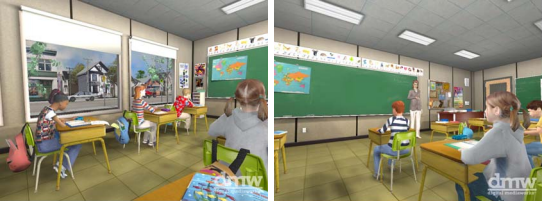
\includegraphics[height=\imgHeightSmall{}]{img/SoA_Rizzo_VirtualClassroom_Cleaned.PNG}}
			\captionof{figure}{Salle de classe virtuelle (Rizzo \textit{et al.})}
			\label{Rizzo_VirtualClassroom}
		\end{minipage}\medskip

		Le matériel utilisé était un HMD avec vision stéréoscopique et capteurs de mouvements ainsi que d'autres capteurs de mouvements sur les bras et les jambes. Ils servent à quantifier le nombre de mouvements de l'enfant et ainsi offrir une métrique supplémentaire.
		
		Un autre outil, développé pour les mêmes raisons que le projet précédent, est le AULA test par Nesplora \cite{Diaz_AulaVRTest}. 
		Son intérêt est l'utilisation du HMD pas uniquement comme périphérique d'affichage mais également comme capteur de mouvements pour quantifier l'attention de la personne (le nombre de mouvements, leur fréquence, mais aussi le temps passé à regarder autre chose). Il ne nécessite donc pas d'autres capteurs de mouvements. La validité de ce test a été étudiée sur un échantillon de 57 enfants (29 sur ce test et 28 sur un test classique) et jugée utile pour compléter un diagnostic de troubles de l'attention.

	\subsection*{VR utilisé pour évaluer l'héminégligence spatiale}

		L'héminégligence spatiale est un des problèmes neurologique le plus étudié à l'aide de la VR (pour l'évaluation et la réhabilitation). Ce trouble apparaît souvent suite à un AVC (Accident Vasculaire Cérébral). Il implique une inattention, ou de la difficulté à répondre aux stimuli apparaissant de l'autre côté de l'hémisphère lésé du cerveau \cite{VARSG4HC1}.
		Katz \textit{et al.} \cite{Katz_CrossStreet} ont réalisé un programme où le patient doit traverser une route dans une réalité virtuelle (figure \ref{Katz_CrossRoad}). Ils ont obtenu des résultats concluant sur l'efficacité de la VR dans le traitement de ce dysfonctionnement. L'asymétrie entre leur angle de déviation ainsi que leur temps de réaction à un stimulus visuel ou auditif sont des métriques pouvant être utilisées pour mesurer le progrès d'un patient.
		
		\begin{minipage}{\linewidth}
			\makebox[\linewidth]{
				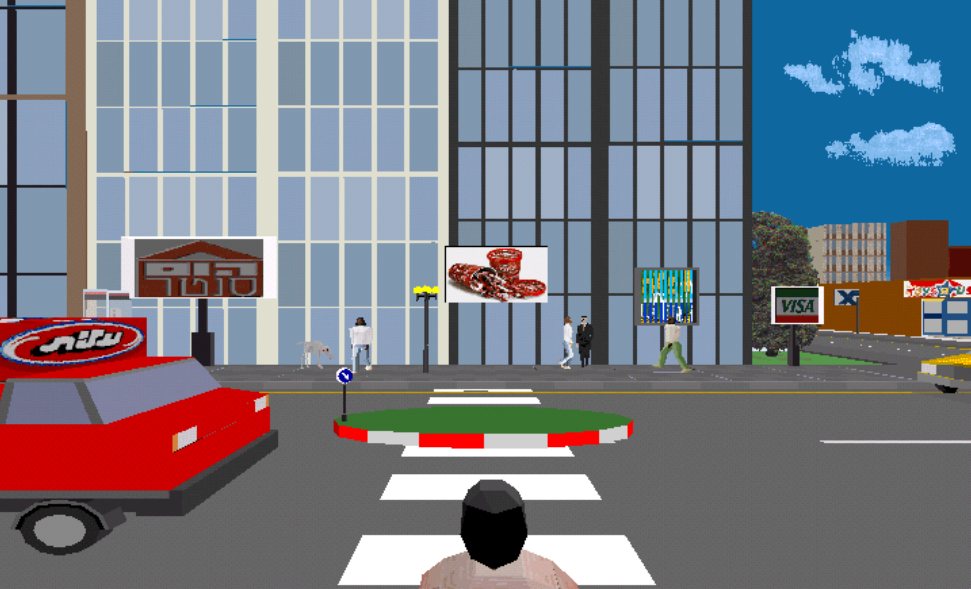
\includegraphics[height=\imgHeightSmall{}]{img/SoA_Katz_CrossRoad.PNG}}
			\captionof{figure}{Environnement virtuel recréer pour simuler la tâche "traverser une route" (Katz \textit{et al.})}
			\label{Katz_CrossRoad}
		\end{minipage}\medskip
		
		%TODO: Lire "Katz_CrossStreet" et étoffer

\section{Simulation 3D en neuropsychologie et neuroréhabilitation suite à un AVC}	
	\label{sSoaSim3DNeuropsyNeuroRehabAVC}
	Entre 30 et 66\% des personnes atteintes d'un AVC ne sont plus capables de se servir de l'un de leur bras dû aux lésions créées dans le cortex cérébral \cite{VanderLee_ForcedUse}. Le succès d'une neuroréhabilitation est directement lié à une grande quantité de mouvements du membre parétique (plus de 20 heures pour une amélioration significative) d'après Cochrane \cite{Cochrane_Intervention4MotorApraxia}). Ils sollicitent la neuroplasticité du cerveau, qui est sa capacité à créer, modifier et détruire des connexions entre les neurones \cite{Grefkes_CorticalReorganization}.

	Les systèmes de VR, pour la neuroréhabilitation cognitive et motrice suite à un AVC, sont en train de se répandre rapidement et de nombreuses plateformes sont en cours de développement. 
	Les avantages de l'utilisation de la réalité virtuelle qui peuvent être trouvés dans la littérature scientifique sont les suivants \cite{VARSG4HC1}:
	\begin{itemize}
		\item \textbf{Neuroplasticité --} Permet l'utilisation de scénarios basés sur des principes facilitant la neuroplasticité tels que l'intensité d'un exercice, sa fréquence, etc.;
		\item \textbf{Entraînement personnalisé --} Offre la possibilité au thérapeute de pouvoir personnaliser l'intensité et la difficulté de l'entraînement d'après les besoins du patient;
		\item \textbf{Objectifs motivants --} L'exercice peut définir des tâches ayant pour but de ré-entraîner des capacités spécifiques (\textit{e.g.}, atteindre un objet, le saisir) tout en étant dans un scénario ludique afin de maintenir une grande implication du patient; %TODO: Parler de ça ?: In particular, al of sutdies evidenced the of VR in augmenting the sense of Presence[49, 50] and the optimal experience [25] in the rehabilitative process.
		\item \textbf{Mesures quantitatives --} À l'aide de capteurs intégrés aux systèmes de réalité virtuelle, il est possible d'avoir un enregistrement précis des actions effectuées par le patient et de se servir de ces informations pour mesurer les performances et le progrès;
		\item \textbf{Entraînement d'activité de la vie quotidienne --} La réalité virtuelle permet la réalisation d'exercices de réhabilitation dans un scénario de tâches de la vie quotidienne (\textit{e.g.}, payer au supermarché).	
	\end{itemize}
	%TODO: Mettre ça ?: The capacity of VR-based systems as a facilitation tool for functional recovery by engaging brain circuits, such as motor areas, has been demonstrated [2].

	Une méta-analyse a été réalisée par Saposnik et Levin \cite{Saposnik_VR4StrokeRehab} sur 12 études (195 participants) afin de déterminer les bénéfices de l'utilisation de la VR pour le rétablissement de la motricité du bras (suite à un AVC). Les résultats obtenus ont permis de montrer que l'ajout d'exercices de réalité virtuelle dans une thérapie augmente son efficacité.
	\\
	
	Dans cette section sont présentés plusieurs plateformes de VR pour la réhabilitation des membres supérieurs et de la main.

	%TODO: Placer ça dans l'intro aussi? : "In the last decade, the use of VR in neurorehabilitation rose a significant way and a n increasing number of experimental findings suggested that this technology can positively impact upon cognitive and motor functional recovery [1-3, 33, 37, 52, 57]. The rationale for the use of VR systems in the rehabilitation field is based on a series of advantages widely documented in the scientific literature:

	\subsection*{Broeren \textit{et al.} - VR et haptique, réhabilitation motrice du bras d'un patient}
		Broeren \textit{et al.} \cite{Broeren_VRHaptic} ont étudié si un environnement virtuel couplé à un périphérique haptique peu augmenter les fonctions motrices d'un bras parétique de sujets ayant subis un AVC. Le système consiste en un joystick 3D avec retour de force (translations et rotations) ainsi qu'un écran stéréoscopique (avec lunettes) pour afficher l'EV en 3D (figure \ref{Broeren_System}).
		
		Le but du programme est de frapper une balle afin qu'elle casse des briques pour gagner des points dans une zone en 3D. Si la balle n'est pas renvoyée, le patient perd des points. L'environnement 3D contient la balle, des briques et un affichage du score, le tout étant à l'intérieur d'un cube. 
		
		L'étude est basée sur un sujet et un groupe de contrôle de 9 personnes saines d'une moyenne de 50 ans. Elle a été effectuée sur quatre semaines où 12 sessions de 90 minutes ont été effectuées. Elle a montré une amélioration de la dextérité et de la force, jugées utiles dans des applications quotidiennes par le patient.
		
		\begin{minipage}{\linewidth}
			\makebox[\linewidth]{
				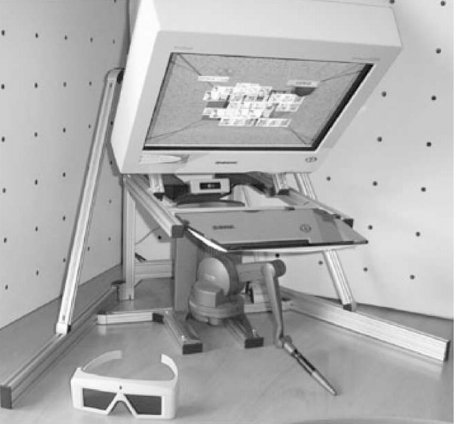
\includegraphics[height=\imgHeightSmall{}]{img/SoA_Broeren_SystemHaptic.PNG}}
			\captionof{figure}{Broeren \textit{et al.} - Système haptique avec vision stéréoscopique utilisé.}
			\label{Broeren_System}
		\end{minipage}\medskip

	\subsection*{Crosbie \textit{et al.} - VR pour la réhabilitation du bras suite à un AVC}
		Le système développé par Crosbie \textit{et al.} \cite{Crosbie_DevVR4StrokeRehab} utilise un HMD (CyVisor) avec des écouteurs intégrés qui affiche un environnement virtuel composé d'objets simples et familiers. Il utilise également un gant "5DT data glove" pour faciliter l'interaction manuelle ainsi que des capteurs de position et d'orientation à quatre endroits du corps du patient: trois sur le bras et un sur le HMD pour augmenter l'immersion (figure \ref{Crosbie_Devices}).
		
		\begin{minipage}{\linewidth}
			\makebox[\linewidth]{
				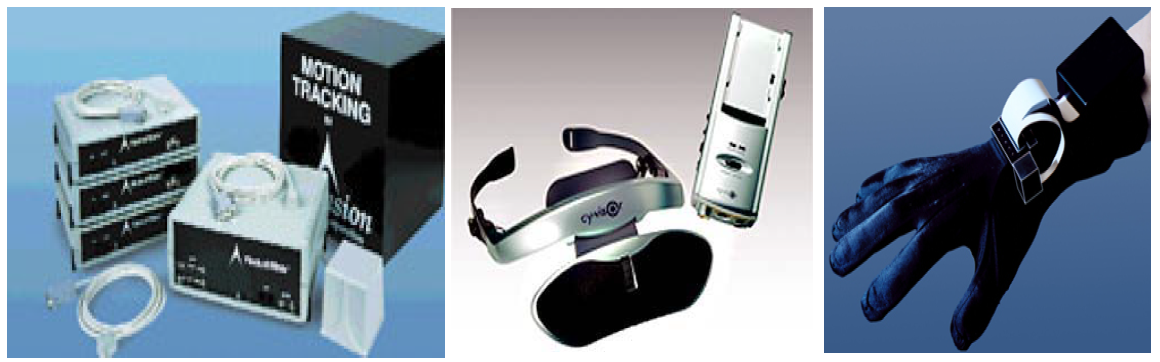
\includegraphics[height=\imgHeightSmall{}]{img/SoA_Crosbie_Devices.PNG}}
			\captionof{figure}{Périphériques utilisés pour l'exercice de réhabilitation (Crosbie \textit{et al.})}
			\label{Crosbie_Devices}
		\end{minipage}\medskip
		
		Le patient est immergé dans l'environnement virtuel où une copie de la table est présente. Il contient également de nombreux objets ainsi qu'une représentation de son bras. Il est alors demandé à l'utilisateur de saisir ces objets et de les déplacer (figure \ref{Crosbie_VE}).

		\begin{minipage}{\linewidth}
			\makebox[\linewidth]{
				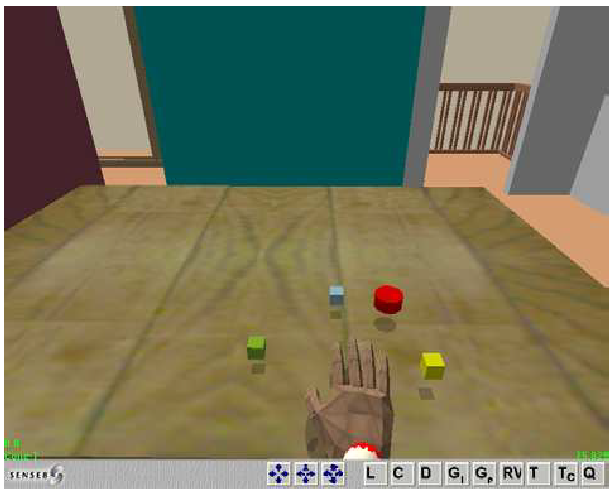
\includegraphics[height=\imgHeightSmall{}]{img/SoA_Crosbie_VE.PNG}}
			\captionof{figure}{Environnement virtuel avec table, objets et représentation du bras (Crosbie \textit{et al.}).}
			\label{Crosbie_VE}
		\end{minipage}\medskip
		
		Tous les éléments du système ainsi que les interactions de l'utilisateur sont mesurables. La réhabilitation peut alors être quantifiée sur la base de ces mesures.
		
		Une étude avec deux groupes de sujets a été menée \cite{Crosbie_RandomizedStudy}. Le premier groupe a effectué une réhabilitation avec ce système et le deuxième, une réhabilitation traditionnelle. Les mesures des capacités motrices n'ont pas montré de différences effectives entre les groupes. L'étude a donc montré l'utilisation possible de la réalité virtuelle pour ce cas de réhabilitation. Si les résultats ne sont pas meilleurs, ils sont cependant plus complets (grâce à l'enregistrement des mouvements de l'utilisateur) pour de futures analyses.
		
		Une autre étude \cite{Crosbie_UserPerpective} a également été réalisée auprès des utilisateurs afin d'analyser la qualité de l'immersion et l'effort ressenti avec, notamment, l'échelle de Borg. L'utilisation de la réalité virtuelle peut en effet provoquer chez certaines personnes des nausées, maux de tête et vertiges.
		%TODO: Semble non finit

	\subsection*{Boian \textit{et al.} VR pour la réhabilitation des mains}
		Le système de VR réalisé par Boian \textit{et al.} pour la réhabilitation des mains \cite{Boian_HandRehab} utilise un \textit{CyberGlove} et un gant haptique "\textit{Rutgers Master II-ND}". Le but de ce système étant d'augmenter la plage de mouvement, la vitesse, l'indépendance et la force de chaque doigt (figure \ref{HapticGlove}).
		
		Une étude a été réalisée \cite{MeriansSensorimotorTraining} pour tester l'efficacité des entraînements utilisant ce système. Les mesures effectuées sur les huit sujets ont montré une amélioration de la plage de mouvement des doigts, de leur force, de leur capacité à bouger indépendamment et de leur vitesse. Leur conclusion est qu'il est difficile qu'un patient ai suffisamment de pratique pour améliorer ses capacités, c'est pourquoi l'utilisation de la VR peut être une bonne solution pour maximiser le temps du patient et du thérapeute.


		\begin{minipage}{\linewidth}
			\makebox[\linewidth]{
				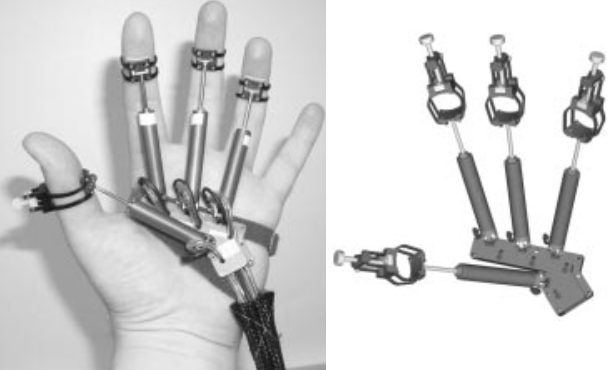
\includegraphics[height=\imgHeightSmall{}]{img/SoA_Boian_HapticGlove.PNG}}
			\captionof{figure}{Rutgers Master II-ND, gant avec retour de force.}
			\label{HapticGlove}
		\end{minipage}\medskip
		
		Pour chacune de ces caractéristiques, un exercice est réalisé dans une réalité virtuelle. Ils comprennent une représentation de la main ainsi que d'autres éléments sur un fond vert. Le gant haptique n'est utilisé que pour la force, les autres exercices utilisaient le \textit{CyberGlove} (figure \ref{Boian_VR}).
		
		\begin{minipage}{\linewidth}
			\makebox[\linewidth]{
				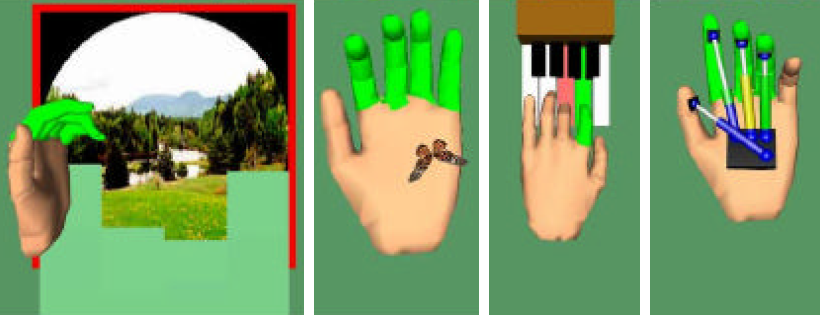
\includegraphics[height=\imgHeightSmall{}]{img/SoA_Boian_VR_FlatCleaned.PNG}}
			\captionof{figure}{Boian \textit{et al.} - Aperçu des exercices. Dans l'ordre de lecture: Plage de mouvement; vitesse; indépendance; force.}
			\label{Boian_VR}
		\end{minipage}\medskip
		
		Sur quatre patients, tous ont significativement amélioré l'indépendance de leurs doigts (possibilité d'en bouger un individuellement), trois ont augmentés leurs vitesses et leurs plages de mouvement. Le gain en force était relativement faible dû à une malfonction du gant.

\section{SGs pour la réhabilitation d'un membre suite à un AVC}

	\label{sSoaSGNeuroRehab}
%TODO: Parler de ça ?: In particular, there is evidence for the effectiveness of such approaches for the rehabilitation of upper limbs in patients with stroke [14, 31, 37, 57]."
	Comme expliqué dans la section précédente, pour qu'une réhabilitation soit efficace, il faut beaucoup de pratique et des exercices répétés. La thérapie en elle-même peut alors être vue comme ennuyante même si elle se déroule dans une réalité virtuelle. L'ajout d'éléments ludiques se prête bien aux thérapies utilisant la réalité virtuelle (l'immersion dans un environnement virtuel et différents périphériques d'interaction déjà présents). Ces éléments ludiques peuvent ajouter de l'intérêt à ces exercices. Mais la motivation, qui est un des facteurs clés des systèmes utilisant la réalité virtuelle pour la réhabilitation \cite{Robertson_AugmentedFeedback}, peut être largement augmentée dans le cas d'un jeu sollicitant ces exercices pour progresser. Les personnes effectuant une réhabilitation apprécient le challenge \cite{Burke_DesigningEngagingPlayableGames4Rehab}, or il est rarement présent dans les thérapies classiques ou les exercices simples en réalité virtuelle. De plus, le côté ludique ne concerne plus uniquement de petits éléments de l'exercice. C'est l'exercice qui, aux yeux du patient, doit être un élément du jeu. C'est le principe des \textit{serious games} (SG) qui peuvent comporter toutes les mécaniques d'un jeu habituel appliquées à un aspect sérieux. Dans cette section sont présentés différents SG où l'aspect sérieux est la pratique d'exercices de réhabilitation. Ainsi, la thérapie, qui pouvait être vue comme une série longue et répétitive de mouvements, peut être perçue comme une activité agréable. De nombreux jeux actuels arrivent à maintenir le joueur engagé durant de longues périodes malgré que l'interaction ne se base que sur quelques boutons appuyés de façon répétitive.
	L'utilisation de robots pour assister les mouvements est l'une des approches prometteuses pour les patients avec une atteinte modérée ou sévère de la motricité. Ils permettent d'accompagner le patient s'il ne fournit pas une force suffisante ou de corriger ses mouvements si nécessaire. Ils permettent également de mesurer les détails des mouvements du patient pour mesurer sa progression.

	\subsection*{\textit{ARMin} et SGs} 
		"\textit{ARMin}" \cite{Nef_ARMinRobot} est un exosquelette robotisé permettant de bouger les articulations de l'épaule, du coude et du poignet (figure \ref{Nef_ARMin}).
		
		\begin{minipage}{\linewidth}
			\makebox[\linewidth]{
				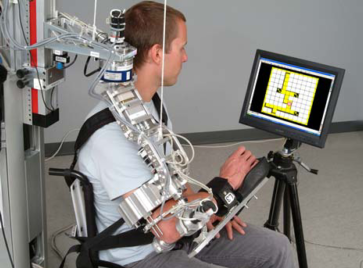
\includegraphics[height=\imgHeightSmall{}]{img/SoA_Nef_ARMin.PNG}}
			\captionof{figure}{Robot \textit{ARMin}, robot de réhabilitation développé à l'\textit{ETHZ}.}%TODO: Expliquer ce qu'est l'ETHZ ? Le mettre dans le lexique ?
			\label{Nef_ARMin}
		\end{minipage}\medskip
		
		Il est couplé à un écran et des haut-parleurs et permet de réaliser des exercices (non détaillés dans ce rapport) et deux jeux pour la réhabilitation du bras (figure \ref{Nef_Scenarios}). Dans le premier jeu, une boule se déplace d'après les mouvements du bras du patient. Le but étant d'amener la boule en haut du labyrinthe, la balle ne devant pas toucher les bords. Dans le deuxième jeu, le patient déplace une poignée à l'écran afin d'attraper une boule qui tombe. La poignée passe du rouge au vert et un \textit{feedback} sonore se produit si le patient attrape la balle.
		
		\begin{minipage}{\linewidth}
			\makebox[\linewidth]{
				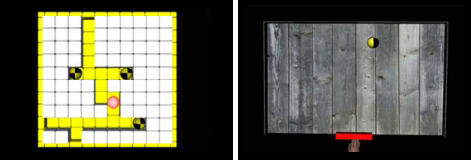
\includegraphics[height=\imgHeightSmall{}]{img/SoA_Nef_Selection.PNG}}
			\captionof{figure}{Fenêtres des jeux de l'\textit{ARMin}. Dans l'ordre de lecture: jeu du labyrinthe; jeu de la boule.}
			\label{Nef_Scenarios}
		\end{minipage}\medskip
		
		L'assistance du robot ou sa résistance peut être réglée par le thérapeute.
		Plusieurs études sans groupe de référence ont tout de même montré qu'une grande utilisation du système peut significativement améliorer les capacités du patient \cite{Nef_EffectsArmTraining, Staubli_EffectsIntensiveArmTraining}.



%"Robotic rehabilitation systems help guide hemiparetic movements actively if adequate motor control is unavailable and show particular promise for patients who may have more severe upper limb impairments [78]."

%TODO Parler de cette étude ? Les jeux ont vraiment l'air trop basique pour être intéressant. Rien de nouveau par rapport à ARMin et SGs...
%\subsection*{UL-EX07 et SGs}
%"In Kim \textit{et al.} [55] the UL-EX07 robot was combined with eight interactive video games as an intervention for 30 hemiparetic participants." "Four of the games developed for this study were purely diagnostic tools; these included flower, paint, joint movement and reach. The remaining four: "pong", "cirular pong", "pinball" and "hand ball" games, were all able to accommodate either bimanual of unilateral therapeutic movements. Difficulty using the UL-EX07 is modulated by adjusting the level of compensation for gravity and active assistance provided by the robot."

%TODO Parler de cette étude ? Les jeux ont vraiment l'air trop basique pour être intéressant. Rien de nouveau par rapport à ARMin et SGs...
%subsection*{Plasma pong, Hummingbird, Virtual Piano, Hammer Task}
%Merians \textit{et al.} [80] ont fait une étude avec des Cyberglove et CyberGrasp (exosquelette robotique pour les doigts). 4 jeux ont été testés :
%Plasma pong
%Hummingbird
%Virtual Piano
%Hammer Task

%TODO Parler de ça ? (Aucune info sur les jeux trouvée...)
%"In Housman \textit{et al.} [50] the results of an intervention using a passive robotic exoskeleton called T-WREX combined with Vu Therapy games was reported in chronic stroke participants. ... Prior to each session Vu Therapy games undergo a software-based calibration by a clinician which adjusts difficulty accordingly."

%TODO Parler de cette étude ? Les jeux ont vraiment l'air trop basique pour être intéressant. Rien de nouveau par rapport à ARMin et SGs...
%Steinisch \textit{et al.} [111] a fait un étude avec un robot passif et 5 jeux vidéos ("Sponge", "Bug hunt", "Twirl", "Grab 2D", "Grab 3D".










%18.5 Virtual Reality and Custom Upper Limb Video Games

% TODO: Trouver où placer ce blabla écologique (du chap 18): "First, the use of rich, multisensory, graphical representations of real world scenarios can provide a more cognitively stimulating and salient experience for the patient. Second, task practice in a simulated environment may provide more ecological validity than practice performed in conventional therapy sessions [100]." 
% TODO: Trouver où placer ce blabla cyber sickness (du chap 18) "Fully immersive systems commonly use head mounted displays thar are sometimes associated with cyber sickness in the elderly population [6, 70]." 

%TODO: Parler d'eux peu-être. Peu d'info on été trouvé sur les jeux en soi. : Sucar \textit{et al.} [113] ont fait une étude comparative entre les thérapies conventionel et un système de jeux vidéos. 8 jeu demandant des taches et mouvements spécifiques.

	\subsection*{Ma et Bechkoum - SGs pour une thérapie basée sur le mouvement suite à un AVC}
		Le but de ce projet est d'encourager les patients à faire leur thérapie de mouvement pour la réhabilitation de leur bras parétique. Ceci est réalisé à l'aide d'un ensemble de SGs où des facteurs tels que la taille des éléments ou la gravité peuvent être réglés afin de s'adapter à leurs capacités \cite{Ma_SG4MovTherapy}. Tous les SGs utilisent un environnement virtuel immersif à l'aide d'un HMD ainsi qu'un retour sonore.
		\\

		\textbf{\textit{Catch-the-orange} --} Dans ce SG, le patient doit ramasser des oranges qui tombent d'un arbre (figure \ref{Ma_CatchOrange}, image de gauche) à l'aide d'un panier. La position et l'orientation du panier sont obtenues via un capteur posé sur un panier réel que le patient doit tenir avec une ou deux mains, en fonction de la thérapie (figure \ref{Ma_CatchOrange}, image de droite). Si le panier est au mauvais endroit, les oranges tombent par terre et sont perdues. S'il est trop incliné celles déjà ramassées peuvent tomber et être également perdues.
		La difficulté est réglable via: un facteur de gravité; la taille des oranges; le laps de temps qui s'écoule entre chaque chute d'orange.
		
		\begin{minipage}{\linewidth}
			\makebox[\linewidth]{
				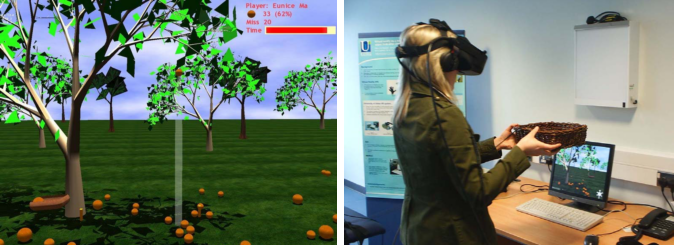
\includegraphics[height=\imgHeightSmall{}]{img/SoA_Ma_CatchOrange.png}}
			\captionof{figure}{Ma et Bechkoum - \textit{Catch-the-orange}. Dans l'ordre de lecture: environnement virtuel; individu en train de jouer.}
			\label{Ma_CatchOrange}
		\end{minipage}\medskip
		
		\textbf{\textit{Fishing game} --} Ce SG est celui le plus apprécié par les patients. Ils sont immergés dans un monde sous-marin et doivent se servir de leurs bras pour attraper des poissons qui nagent (figure \ref{Ma_Fishing}, image de gauche). Le patient voit une représentation de ses deux mains, ce qui est rendu possible grâce à l'utilisation d'un capteur par main (figure \ref{Ma_Fishing}, image de droite). Si une main touche le poisson, il partira en nageant bien plus vite. Cependant, si les deux mains le touchent, il se débattra (retour visuel) puis disparaîtra en incrémentant le compteur de poissons attrapés. La difficulté est réglable via: la taille de la zone (amplitude du mouvement); la vitesse des poissons; leur taille; la taille des mains.

		\begin{minipage}{\linewidth}
			\makebox[\linewidth]{
				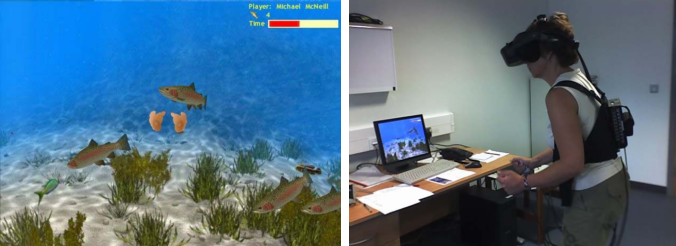
\includegraphics[height=\imgHeightSmall{}]{img/SoA_Ma_Fishing.png}}
			\captionof{figure}{Ma et Bechkoum - \textit{Fishing game}. Dans l'ordre de lecture: environnement virtuel; individu en train de jouer.}
			\label{Ma_Fishing}
		\end{minipage}\medskip
		
		\textbf{\textit{Whack-a-mouse} --} En plus d'améliorer la mobilité, la précision et la vitesse du bras, ce SG a été conçu pour améliorer la discrimination visuelle et l'attention sélective. Ce sont des facteurs importants d'une réhabilitation suite à un AVC pour les patients présentant une héminégligence spatiale. Dans ce SG, une souris apparaît sur une table à un endroit aléatoire et y reste, un certain nombre de secondes, puis disparaît pour réapparaître ailleurs. Le joueur doit frapper la souris avec un marteau contrôlé par la position et l'orientation d'un capteur sur sa main (figure \ref{Ma_Mouse}). Quand la souris est touchée, elle fait en petit cri et devient rouge (retour visuel) avant d'incrémenter le score. La difficulté est réglée via le nombre de secondes où la souris reste.

		\begin{minipage}{\linewidth}
			\makebox[\linewidth]{
				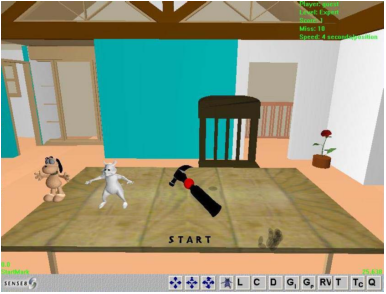
\includegraphics[height=\imgHeightSmall{}]{img/SoA_Ma_WhackAMouse.png}}
			\captionof{figure}{Ma et Bechkoum - \textit{Whack-a-mouse}, environnement virtuel.}
			\label{Ma_Mouse}
		\end{minipage}\medskip

		Les jeux se règlent automatiquement par rapport au profil du patient. Les paramètres cités dans chaque jeu mais également le lieu des stimuli, se règlent en fonction (prenant compte également du côté parétique et de son héminégligence). Des niveaux de difficulté "facile", "intermédiaire" et "expert" sont disponibles. Dans le niveau facile le jeu s'adapte simplement au profil du patient. Dans le niveau intermédiaire, les paramètres changent en cours de partie (plus le patient a du succès, plus la difficulté augmente et inversement). Le niveau expert utilise des éléments malus. Exemple: dans \textit{Whack-a-mouse}, un chien apparaît en même temps que la souris et le joueur ne doit pas se tromper de cible, ce qui fait travailler sa discrimination visuelle.
		\\
		
		Le niveau, le score et la vitesse sont affichés constamment en haut à gauche et, en fin de partie ou en passant au niveau suivant, des informations telles que le score, la précision moyenne et la durée sont affichées sur un écran final. Ces données sont également enregistrées dans un fichier pour régler la difficulté lors de prochaines parties ou pour que le thérapeute les analyse. Pour créer un peu de compétition, le patient peut voir les meilleurs scores de tous les joueurs mais également juste les siens pour chaque niveau et chaque jeu.
		\\
		
		Des tests utilisateurs ont été réalisés sur huit patients entre 43 et 75 ans. Un groupe (quatre patients) faisait une thérapie de mouvement traditionnelle et des SGs et l'autre ne faisait pas les SGs. Il n'est pas précisé la durée des sessions pour chaque groupe. Les tests ont montré un impact positif de l'utilisation des SGs pour améliorer les capacités motrices.

%TODO: Doc non trouvable gratuitement (demande effectuée). Si trouvée, ecrire là dessus
%Crosbie \textit{et al.} ont continuer à faire des SG [23] ("Rabbit chase", "Arrow Attack")

%TODO: Doc non trouvable gratuitement Si trouvée, ecrire là dessus
%TODO: Documenter au moins le produit utilisé -> 20 jeux pour différentes pathologies ! (http://www.gesturetekhealth.com/products-rehab-irex.php)
%Kwon \textit{et al.} [62] ont fait un étude avec un outils clinique de VR "IREX" dévelopé par GestureTek et qui offre 23 jeux de réhabilitation dont 5 pour la réhabilitation des membres supérieurs. Il se sert d'une caméra et de Cybergloves pour capter les mouvements. Le système fournit une variété de feedback incluant des scores ainsi que des diagrammes de progression.

%TODO: Attendre la récéption du 18_89 (demandé via research gate) et éventuellement écrire un truc dessus (semble un peu simple comme jeu)
%\subsection*{Rehabilitation Gaming System}
%"Rehabilitation Gaming System" est développé d'après un projet scientifique, par une collaboration entre des universités et des hôpitaux en Espagne. 
%http://rgs-project.eu/games
%The Rehabilitation Gaming System (RGS) is a novel and highly innovative ICT Virtual Reality (VR) tool for the rehabilitation of motor deficits of the upper extremities after a brain lesion due to stroke. The system deploys an individualized game training that combines movement execution with the observation of a correlated action by virtual limbs that are displayed in a first-person perspective. (read more description below)
%Cameirao et al on fait une étude avec "Rehabilitation Gaming System" [15, 89] se servant de "Data glove" pour récupérer les flexions des doigts

	\subsection*{\textit{Voracy Fish} \cite{VoracyFish}}%Le projet MoJOS n'existe plus. Même l'adresse http://www.mojos.fr/home/ redirige sur http://www.voracy.com/
		Ce projet a également pour but la réhabilitation du bras chez les personnes ayant eu un AVC. Il est créé par \textit{Brain  e-NOVATION} \cite{BrainENOVATION} étant un laboratoire mettant en commun l'expertise médicale de "l'Institut du Cerveau et de la Moelle Épinière" (ICM) et l'expertise informatique orientée santé du groupe français \textit{GENIOUS}. Le SG se joint à la plateforme \textit{GENIOUS GAMe-S} proposant un espace patient et un espace thérapeute avec une liaison directe entre les exercices effectués par le patient chez lui et l'hôpital pour que le thérapeute puisse voir d'une part la progression et d'autre part lui communiquer des informations, planifier des séances ou directement changer la rééducation. Ce projet a été récompensé à de nombreuses reprises, notamment par un trophée e-santé en 2013 pour son travail dans la catégorie "Autonomie et maintien à domicile", en étant finaliste "e-virtuoses" en 2013 dans la catégorie "\textit{serious game} Santé", ou encore par le titre de meilleur projet industriel "e-santé" 2012.
		\\
		
		Pour le matériel, les mouvements du patient sont récupérés à l'aide d'une \textit{Kinect} (caméra développée par Microsoft permettant la reconnaissance d'un mouvement du corps dans un environnement en 3D \cite{Kinect_website}), le jeu est affiché sur un écran et des haut-parleurs sont présents pour l'audio (figure \ref{FigVoracyFish}, image de droite). Le patient peut effectuer les mouvements en l'air ou le bras posé sur une table. Il peut également guider son bras parétique avec son autre bras si besoin. L'avantage de cette solution est qu'elle utilise des dispositifs tout public et permet la réalisation des exercices à la maison.
		\\
		
		Dans le jeu, le patient incarne un poisson dans un environnement 3D contenant des éléments audio (figure \ref{FigVoracyFish}, à gauche). Son but étant de manger d'autres poissons et de trouver des trésors. Plus il mange de poissons, plus il grandit et plus il monte dans la chaîne alimentaire et peut manger de plus gros poissons. Le poisson se déplace constamment et le joueur peut influer sur la direction (verticale et horizontale) à l'aide de la position de son bras.
		\\
		
		Ce jeu peut également se jouer à plusieurs joueurs et avec d'autres périphériques d'entrée, tels qu'une tablette tactile ou une souris. Le but du joueur est alors de manger ses adversaires. Ainsi le patient peut effectuer sa thérapie (avec la \textit{Kinect} \cite{Kinect_website}) à la maison tout en s'amusant avec ses proches (qui utilisent une tablette ou une souris).\medskip
		
		\begin{minipage}{\linewidth}
			\makebox[\linewidth]{
				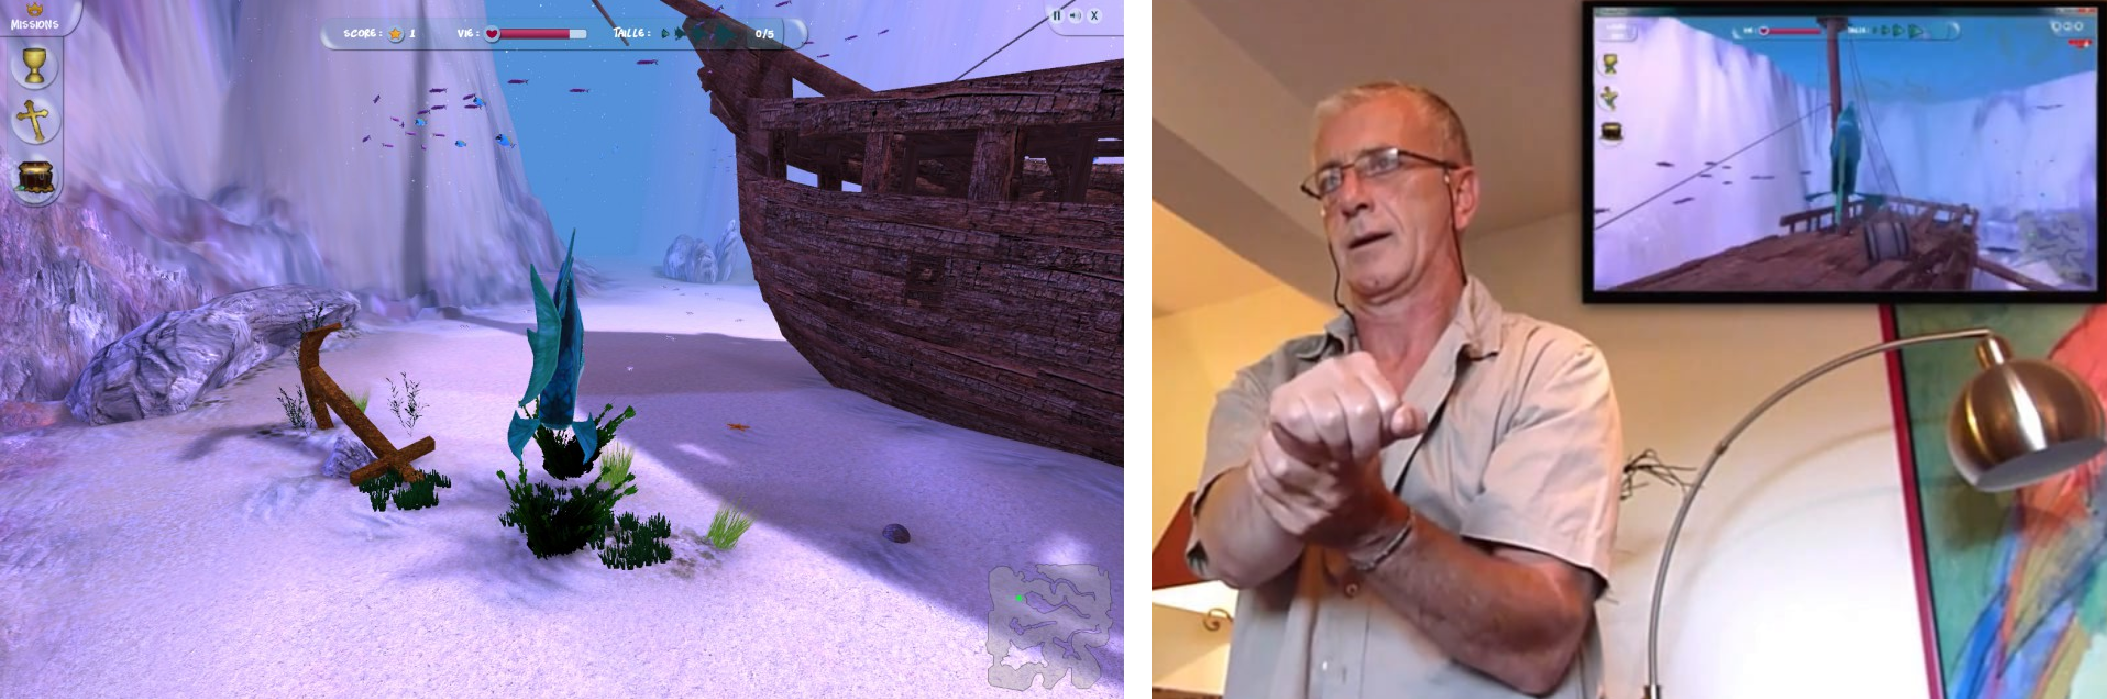
\includegraphics[height=\imgHeightSmall{}]{img/SoA_VoracyFish.png}}
			\captionof{figure}{\textit{Voracy Fish}. Dans l'ordre de lecture: environnement virtuel; individu en train de jouer.}
			\label{FigVoracyFish}
		\end{minipage}\medskip
		
		Aucune d'études clinique n'a encore été effectuée, mais c'est un des prochains objectifs du groupe \textit{Brain e-NOVATION} \cite{ICM_Strokes}.
	
	\subsection*{Neurorehabilitation Training Toolkit (NTT)}
		Ce concept a pour but une réhabilitation motrice des bras à domicile avec une installation à faible coût \cite{Bermudez_NTT}. Il est réalisé par l'université Da Madeira au Portugal et consiste en une application web accessible depuis un navigateur internet pour fournir le SG, les instructions et les retours d'informations. Il exige également que le PC ai deux souris (une extension a, par la suite, été réalisée pour être utilisée avec une \textit{Kinect} \cite{Bermudez_NTTToKinect}). Une souris sera utilisée par main, celles-ci étant posées sur la table, et a donc un support contre la gravité. La réhabilitation se fait à l'aide de mouvements répétitifs dans le but d'augmenter la coordination, la synchronisation des bras et leur précision.
		\\
		
		Dans le jeu, le patient voit son avatar aux commandes d'un parapente (figure \ref{Bermudez_NTT}, image de gauche) et peut contrôler sa direction à l'aide d'une différence de position verticale entre les mains (figure \ref{Bermudez_NTT}, image de droite), comme s'il tirait sur les poignées du parapente. Le parapente avance à vitesse constante, le but étant de collecter le plus de ballons possible. Cette mécanique de jeu est choisi afin que le patient puisse compenser les mouvements réduits et peu précis du bras parétique avec l'autre. Pour le scénario, le joueur doit retrouver sa maison en avançant de niveau en niveau (il faut récupérer assez de ballons pour passer au niveau suivant). Le jeu commence par un tutoriel. Le jeu essaie d'utiliser le plus de repères et de modalités de retour possibles pour s'assurer que l'utilisateur comprenne l'influence de ses actions et ne se perde pas. Par exemple, à l'écran, une boussole montre la direction du prochain ballon et une image montre le mouvement à effectuer pour aller dans cette direction.
		\\
		
		Quatre paramètres peuvent être modifiés pour adapter la difficulté: la vitesse; la vitesse de rotation; la distance minimale pour collecter un objet; la distance entre les objets à collecter.\medskip
				
		\begin{minipage}{\linewidth}
			\makebox[\linewidth]{
				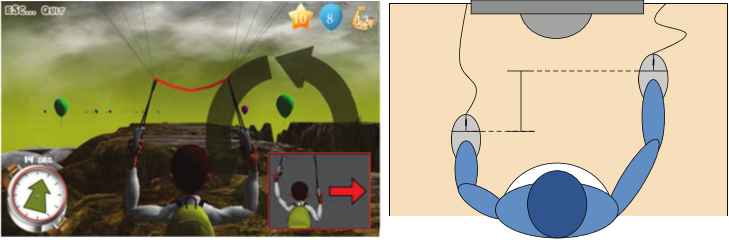
\includegraphics[height=\imgHeightSmall{}]{img/SoA_Bermudez_Edited.png}}
			\captionof{figure}{NTT. Dans l'ordre: interface et environnement virtuel; installation du patient en jeu.}
			\label{Bermudez_NTT}
		\end{minipage}\medskip		
		
	\subsection*{Stroke Recovery with Kinect}
		Ce projet développé par "Microsoft Research"\cite{MicrosoftResearch} consiste en trois programmes de réhabilitation du bras à l'aide d'une Kinect \cite{Microsoft_StrokeRecovery}. Les programmes sont les suivants:
		\begin{itemize}
			\item Un test classique où le patient doit prendre des blocs et les mettre dans une boîte en un temps donné, réalisé dans une réalité virtuelle (figure \ref{MicrosoftResearch_StrokeRecovery}, image de gauche). Le plus de cette utilisation est l'établissement direct d'un score après une session de jeu et la visualisation de la progression au fil des parties;
			\item Un exercice où le patient doit imiter les mouvements affichés à l'écran (figure \ref{MicrosoftResearch_StrokeRecovery}, image du centre). Il reçoit un score basé sur son succès d'après l'échelle de Fugl-Meyer, qui est la mesure quantitative la plus utilisée pour mesurer le progrès d'une réhabilitation pour des patients hémiplégiques \cite{FuglMeyerAssesment};
			\item Un SG dans l'espace où le patient entraîne ses réflexes en guidant un vaisseau spatial horizontalement (via des mouvements horizontaux des bras) pour éviter des astéroïdes (figure \ref{MicrosoftResearch_StrokeRecovery}, image de droite).
		\end{itemize}
		Tous les programmes sont affichés sur un écran (pas d'utilisation de HMD).\medskip
		
		\begin{minipage}{\linewidth}
			\makebox[\linewidth]{
				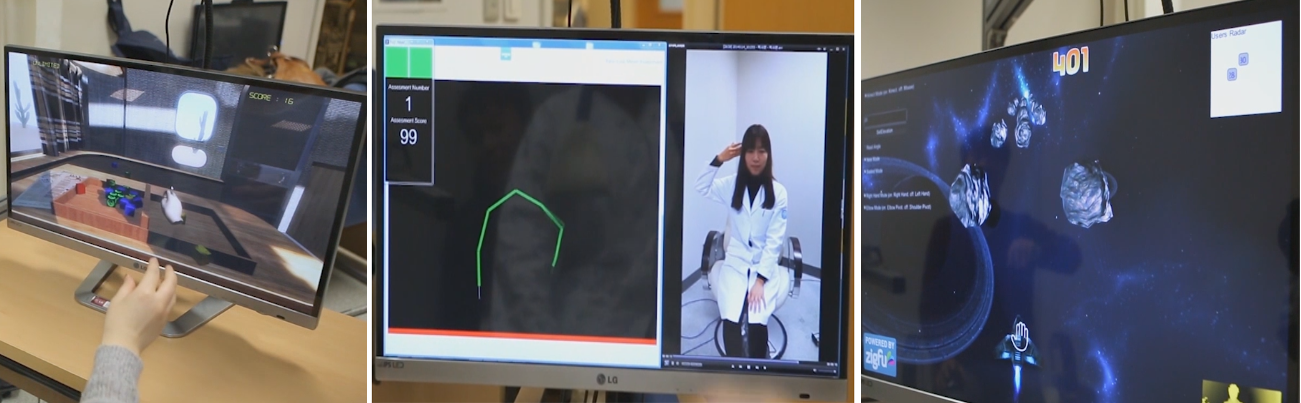
\includegraphics[height=\imgHeightSmall{}]{img/SoA_MicrosoftResearch_StrokeRecovery_Resized.png}}
			\captionof{figure}{Stroke Recovery with Kinect. Dans l'ordre de lecture: test classique; imitation de mouvements; SG.}
			\label{MicrosoftResearch_StrokeRecovery}
		\end{minipage}\medskip
		
		Objectifs à long terme:
		\begin{itemize}
			\item Intégration d'un aspect social pour faire des parties à un contre un et ainsi faire augmenter la motivation;
			\item La construction d'une communauté où ils pourront communiquer leurs problèmes et recevoir des encouragements et de l'aide;
			\item Permettre au personnel médical de contrôler l'avancement des patients depuis leur bureau et de communiquer directement avec eux;
			\item Utilisation d'autres technologies Microsoft, notamment de Cloud pour intégrer du \textit{machine learning}.%TODO: Ajouter dans le lexique ?
		\end{itemize}
		Le point important de ce projet est qu'une référence du domaine informatique tel que Microsoft s'intéresse à ce domaine. Avec de tels moyens, les SGs développés pourront potentiellement être de grande qualité.
				
%\section{SGs pour la réhabilitation des jambes}
	%TODO: Étoffer l'intro
	%Dans cette section est présenté les SGs liés à la neuro-réhabilitation des membres inférieurs, ce sont donc les SGs qui, d’un point de vue but et profil patient sont les plus proche de celui à développer. La complexité de conception pour un SG utilisant les jambes se situe en trois points. Le premier est qu’il est plus difficile de concevoir un jeu avec une interaction basée sur les jambes que sur les bras. Le deuxième point est que les projets cités ne souhaitent principalement réapprendre qu’un mouvement qui est la marche, on ne demande donc aucune autre interaction des membres inférieurs. Le troisième est que si le patient est debout, il doit s’accrocher à des rampes et on exclue alors toute interaction des membres supérieurs.
				
	\subsection*{Gabarello}
		Ce SG est développé pour une utilisation avec le "Lokomat". Ce dernier étant un robot de réhabilitation des jambes contenant principalement un tapis roulant, un exosquelette et un système de soutien du poids du patient développé par \textit{Hocoma} \cite{Lokomat_Brochure} (figure \ref{Lokomat}). Ce SG est destiné essentiellement aux enfants et a été conçu en tant que tel. Le développement a été réalisé par l'université des Arts de Zürich (spécialisation "Game Design") en coopération avec le Kinderspital à Zürich, l'institut de Neuropsychologie de l'université de Zürich et le laboratoire "Sensory Motor Systems Lab" à l'ETHZ.\medskip
		
		\begin{minipage}{\linewidth}
			\makebox[\linewidth]{
				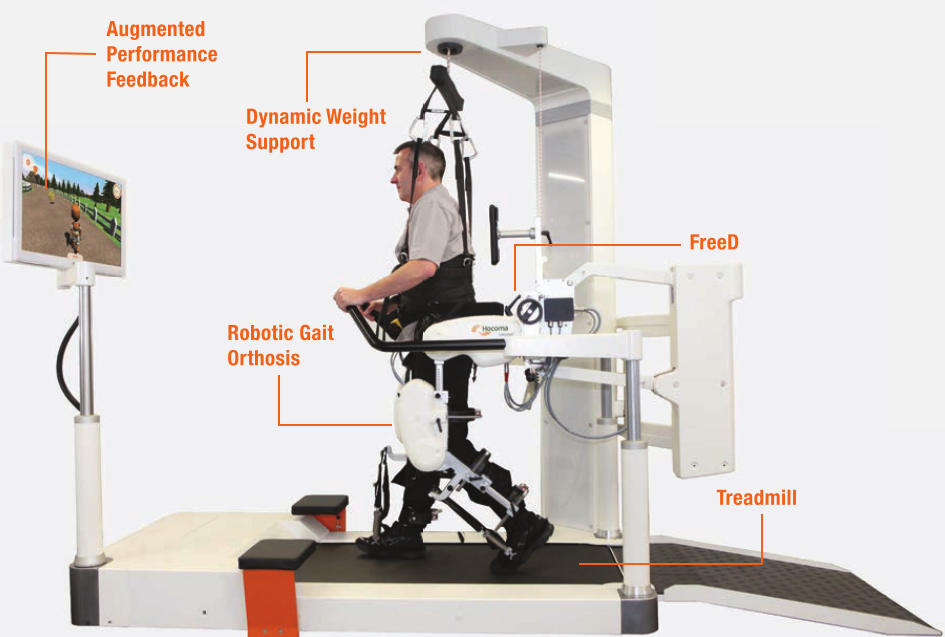
\includegraphics[height=\imgHeightMedium{}]{img/SoA_Lokomat.png}}
			\captionof{figure}{Lokomat, robot de réhabilitation développé par \textit{Hocoma}.}
			\label{Lokomat}
		\end{minipage}\medskip%TODO: Trouver une image avec un enfant du coup ?
		
		Le but du jeu est de collecter des fleurs à la surface d'une planète. Les joueurs contrôlent un astronaute marchant sur celle-ci. En fournissant plus d'effort, les jambes de l'avatar vont grandir (phase active, figure \ref{Gabarello}, image de gauche), et en en fournissant moins, elles vont rapetisser (phase passive, figure \ref{Gabarello}, image de droite). Plus les jambes sont grandes, plus les fleurs récoltées rapportent de points. Avoir de grandes jambes permet aussi de monter sur des plateformes, d'y rester ainsi que de sauter sur les suivantes. L'avatar n'a que trois états qui correspondent au degré d'activité du patient. La synchronisation entre la participation du patient et de l'avatar dure un pas. La force mise par le patient est détectée à l'aide de capteurs directement présents sur le Lokomat \cite{Labruyere_LokomatGabarello}.\medskip
		
		\begin{minipage}{\linewidth}
			\makebox[\linewidth]{
				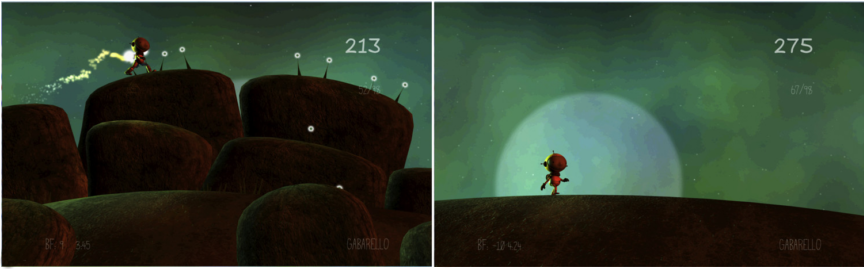
\includegraphics[height=\imgHeightSmall{}]{img/SoA_Lokomat_Gabarello_Cleaned.png}}
			\captionof{figure}{Gabarello. Dans l'ordre de lecture: phase active; phase passive.}
			\label{Gabarello}
		\end{minipage}\medskip
		
		Une étude a été réalisée pour savoir si un enfant peut modifier son niveau de participation pendant un scénario. Les résultats ont montrés qu'il était possible pour eux de modifier leur force durant un exercice, cependant leurs aptitudes cognitives et motrices vont déterminer s'il est capable d'identifier le besoin \cite{Labruyere_LokomatGabarello}.
		\\
		
		D'autres SG fonctionnent avec le Lokomat et font partie du "Challenge package", cependant peu d'informations ont été trouvées \cite{Lokomat_Brochure}. Ils semblent tous se baser uniquement sur le mouvement des jambes (leur synchronisation pour un jeu de vol, la force mise dans le mouvement pour un jeu de course ou encore la trajectoire des pieds) \cite{Lokomat_FlyingGame}. Les jeux semblent contenir des graphismes élaboré, cependant l'interaction de l'avatar et ses déplacements sont saccadés et non cohérent avec son environnement. %TODO Trouver plus d'infos
		
		%TODO Parler de ce projet ou d'un autre (pas faire de sous-section que pour le Lokomat...) :
		%\subsection*{Grail / Stable / CAREN / V-Gait / ...}
		%Projet riche avec beaucoup de périphériques et application dont SG avec de beaux graphismes. Très peu d'infos trouvées sur les SGs...
		
		%http://www.motekmedical.com/products/grail-gait-real-time-analysis-interactive-lab/
		%http://www.motekmedical.com/solutions/rehabilitation/#
